% Options for packages loaded elsewhere
\PassOptionsToPackage{unicode}{hyperref}
\PassOptionsToPackage{hyphens}{url}
%
\documentclass[
]{article}
\usepackage{amsmath,amssymb}
\usepackage{lmodern}
\usepackage{iftex}
\ifPDFTeX
  \usepackage[T1]{fontenc}
  \usepackage[utf8]{inputenc}
  \usepackage{textcomp} % provide euro and other symbols
\else % if luatex or xetex
  \usepackage{unicode-math}
  \defaultfontfeatures{Scale=MatchLowercase}
  \defaultfontfeatures[\rmfamily]{Ligatures=TeX,Scale=1}
\fi
% Use upquote if available, for straight quotes in verbatim environments
\IfFileExists{upquote.sty}{\usepackage{upquote}}{}
\IfFileExists{microtype.sty}{% use microtype if available
  \usepackage[]{microtype}
  \UseMicrotypeSet[protrusion]{basicmath} % disable protrusion for tt fonts
}{}
\makeatletter
\@ifundefined{KOMAClassName}{% if non-KOMA class
  \IfFileExists{parskip.sty}{%
    \usepackage{parskip}
  }{% else
    \setlength{\parindent}{0pt}
    \setlength{\parskip}{6pt plus 2pt minus 1pt}}
}{% if KOMA class
  \KOMAoptions{parskip=half}}
\makeatother
\usepackage{xcolor}
\usepackage[margin=1in]{geometry}
\usepackage{color}
\usepackage{fancyvrb}
\newcommand{\VerbBar}{|}
\newcommand{\VERB}{\Verb[commandchars=\\\{\}]}
\DefineVerbatimEnvironment{Highlighting}{Verbatim}{commandchars=\\\{\}}
% Add ',fontsize=\small' for more characters per line
\usepackage{framed}
\definecolor{shadecolor}{RGB}{248,248,248}
\newenvironment{Shaded}{\begin{snugshade}}{\end{snugshade}}
\newcommand{\AlertTok}[1]{\textcolor[rgb]{0.94,0.16,0.16}{#1}}
\newcommand{\AnnotationTok}[1]{\textcolor[rgb]{0.56,0.35,0.01}{\textbf{\textit{#1}}}}
\newcommand{\AttributeTok}[1]{\textcolor[rgb]{0.77,0.63,0.00}{#1}}
\newcommand{\BaseNTok}[1]{\textcolor[rgb]{0.00,0.00,0.81}{#1}}
\newcommand{\BuiltInTok}[1]{#1}
\newcommand{\CharTok}[1]{\textcolor[rgb]{0.31,0.60,0.02}{#1}}
\newcommand{\CommentTok}[1]{\textcolor[rgb]{0.56,0.35,0.01}{\textit{#1}}}
\newcommand{\CommentVarTok}[1]{\textcolor[rgb]{0.56,0.35,0.01}{\textbf{\textit{#1}}}}
\newcommand{\ConstantTok}[1]{\textcolor[rgb]{0.00,0.00,0.00}{#1}}
\newcommand{\ControlFlowTok}[1]{\textcolor[rgb]{0.13,0.29,0.53}{\textbf{#1}}}
\newcommand{\DataTypeTok}[1]{\textcolor[rgb]{0.13,0.29,0.53}{#1}}
\newcommand{\DecValTok}[1]{\textcolor[rgb]{0.00,0.00,0.81}{#1}}
\newcommand{\DocumentationTok}[1]{\textcolor[rgb]{0.56,0.35,0.01}{\textbf{\textit{#1}}}}
\newcommand{\ErrorTok}[1]{\textcolor[rgb]{0.64,0.00,0.00}{\textbf{#1}}}
\newcommand{\ExtensionTok}[1]{#1}
\newcommand{\FloatTok}[1]{\textcolor[rgb]{0.00,0.00,0.81}{#1}}
\newcommand{\FunctionTok}[1]{\textcolor[rgb]{0.00,0.00,0.00}{#1}}
\newcommand{\ImportTok}[1]{#1}
\newcommand{\InformationTok}[1]{\textcolor[rgb]{0.56,0.35,0.01}{\textbf{\textit{#1}}}}
\newcommand{\KeywordTok}[1]{\textcolor[rgb]{0.13,0.29,0.53}{\textbf{#1}}}
\newcommand{\NormalTok}[1]{#1}
\newcommand{\OperatorTok}[1]{\textcolor[rgb]{0.81,0.36,0.00}{\textbf{#1}}}
\newcommand{\OtherTok}[1]{\textcolor[rgb]{0.56,0.35,0.01}{#1}}
\newcommand{\PreprocessorTok}[1]{\textcolor[rgb]{0.56,0.35,0.01}{\textit{#1}}}
\newcommand{\RegionMarkerTok}[1]{#1}
\newcommand{\SpecialCharTok}[1]{\textcolor[rgb]{0.00,0.00,0.00}{#1}}
\newcommand{\SpecialStringTok}[1]{\textcolor[rgb]{0.31,0.60,0.02}{#1}}
\newcommand{\StringTok}[1]{\textcolor[rgb]{0.31,0.60,0.02}{#1}}
\newcommand{\VariableTok}[1]{\textcolor[rgb]{0.00,0.00,0.00}{#1}}
\newcommand{\VerbatimStringTok}[1]{\textcolor[rgb]{0.31,0.60,0.02}{#1}}
\newcommand{\WarningTok}[1]{\textcolor[rgb]{0.56,0.35,0.01}{\textbf{\textit{#1}}}}
\usepackage{longtable,booktabs,array}
\usepackage{calc} % for calculating minipage widths
% Correct order of tables after \paragraph or \subparagraph
\usepackage{etoolbox}
\makeatletter
\patchcmd\longtable{\par}{\if@noskipsec\mbox{}\fi\par}{}{}
\makeatother
% Allow footnotes in longtable head/foot
\IfFileExists{footnotehyper.sty}{\usepackage{footnotehyper}}{\usepackage{footnote}}
\makesavenoteenv{longtable}
\usepackage{graphicx}
\makeatletter
\def\maxwidth{\ifdim\Gin@nat@width>\linewidth\linewidth\else\Gin@nat@width\fi}
\def\maxheight{\ifdim\Gin@nat@height>\textheight\textheight\else\Gin@nat@height\fi}
\makeatother
% Scale images if necessary, so that they will not overflow the page
% margins by default, and it is still possible to overwrite the defaults
% using explicit options in \includegraphics[width, height, ...]{}
\setkeys{Gin}{width=\maxwidth,height=\maxheight,keepaspectratio}
% Set default figure placement to htbp
\makeatletter
\def\fps@figure{htbp}
\makeatother
\setlength{\emergencystretch}{3em} % prevent overfull lines
\providecommand{\tightlist}{%
  \setlength{\itemsep}{0pt}\setlength{\parskip}{0pt}}
\setcounter{secnumdepth}{-\maxdimen} % remove section numbering
\ifLuaTeX
  \usepackage{selnolig}  % disable illegal ligatures
\fi
\IfFileExists{bookmark.sty}{\usepackage{bookmark}}{\usepackage{hyperref}}
\IfFileExists{xurl.sty}{\usepackage{xurl}}{} % add URL line breaks if available
\urlstyle{same} % disable monospaced font for URLs
\hypersetup{
  pdftitle={Tutorial Rmarkdown},
  hidelinks,
  pdfcreator={LaTeX via pandoc}}

\title{Tutorial Rmarkdown}
\author{}
\date{\vspace{-2.5em}}

\begin{document}
\maketitle

\hypertarget{r-markdown}{%
\subsection{R Markdown}\label{r-markdown}}

This is an R Markdown document. Markdown is a simple formatting syntax
for authoring HTML, PDF, and MS Word documents. For more details on
using R Markdown see \url{http://rmarkdown.rstudio.com}.

It uses \texttt{knitr}, \texttt{rmarkdown} and
\href{http://pandoc.org/}{\texttt{pandoc}}. Pandoc is a universal
document converter, in our case, it goes from:

\textbf{Rmarkdown} =\textgreater{} \textbf{markdown} =\textgreater{}
\textbf{document}

\#\#Syntax \#\#\#Emphasis

\texttt{*italic*} =\textgreater{} \emph{italic}

\texttt{\_italic\_} =\textgreater{} \emph{italic}

\texttt{**bold**} =\textgreater{} \textbf{bold}

\texttt{\_\_bold\_\_} =\textgreater{} \textbf{bold}

\#\#\#Headers

\begin{verbatim}
# Header 1

## Header 2

### Header 3
\end{verbatim}

\#\#\#Lists \#\#\#\# Unordered

\begin{verbatim}
* Item1
  + Item 1a #double tab
* Item 2
\end{verbatim}

\begin{itemize}
\tightlist
\item
  Item1

  \begin{itemize}
  \tightlist
  \item
    Item 1a
  \end{itemize}
\item
  Item 2
\end{itemize}

\hypertarget{ordered}{%
\paragraph{Ordered}\label{ordered}}

\begin{verbatim}
1. Item1
    + Item 1a
2. Item 2
\end{verbatim}

\begin{enumerate}
\def\labelenumi{\arabic{enumi}.}
\tightlist
\item
  Item1

  \begin{itemize}
  \tightlist
  \item
    Item 1a
  \end{itemize}
\item
  Item 2
\end{enumerate}

\hypertarget{links}{%
\subsubsection{Links}\label{links}}

Use plain address either as an actual link, within the text or linked to
a word:

\begin{verbatim}
http://www.fieldcroppathology.msu.edu/
<http://www.fieldcroppathology.msu.edu/>
[Chilvers lab](http://www.fieldcroppathology.msu.edu/)
\end{verbatim}

\url{http://www.fieldcroppathology.msu.edu/}

\href{http://www.fieldcroppathology.msu.edu/}{Chilvers lab}

\hypertarget{images}{%
\subsubsection{Images}\label{images}}

\begin{verbatim}
#If you forgot the exclamation mark (!), it will become just a link
![Chilves lab photo](IMG_8889-Copy.jpg)
\end{verbatim}

\begin{figure}
\centering
\includegraphics{IMG_8889-Copy.jpg}
\caption{Chilves lab photo}
\end{figure}

\#\#\#Tables

\begin{verbatim}
First Header  | Second Header
------------- | -------------
Content Cell  | Content Cell
Content Cell  | Content Cell
\end{verbatim}

\begin{longtable}[]{@{}ll@{}}
\toprule()
First Header & Second Header \\
\midrule()
\endhead
Content Cell & Content Cell \\
Content Cell & Content Cell \\
\bottomrule()
\end{longtable}

You can make this process simpler using knitr with \texttt{kable}:

\begin{Shaded}
\begin{Highlighting}[]
\FunctionTok{kable}\NormalTok{(}\FunctionTok{head}\NormalTok{(ggplot2}\SpecialCharTok{::}\NormalTok{mpg, }\AttributeTok{n =} \DecValTok{15}\NormalTok{), }\AttributeTok{digits =} \DecValTok{3}\NormalTok{, }\AttributeTok{format =} \StringTok{"markdown"}\NormalTok{)}
\end{Highlighting}
\end{Shaded}

\begin{longtable}[]{@{}
  >{\raggedright\arraybackslash}p{(\columnwidth - 20\tabcolsep) * \real{0.1781}}
  >{\raggedright\arraybackslash}p{(\columnwidth - 20\tabcolsep) * \real{0.1507}}
  >{\raggedleft\arraybackslash}p{(\columnwidth - 20\tabcolsep) * \real{0.0822}}
  >{\raggedleft\arraybackslash}p{(\columnwidth - 20\tabcolsep) * \real{0.0685}}
  >{\raggedleft\arraybackslash}p{(\columnwidth - 20\tabcolsep) * \real{0.0548}}
  >{\raggedright\arraybackslash}p{(\columnwidth - 20\tabcolsep) * \real{0.1507}}
  >{\raggedright\arraybackslash}p{(\columnwidth - 20\tabcolsep) * \real{0.0548}}
  >{\raggedleft\arraybackslash}p{(\columnwidth - 20\tabcolsep) * \real{0.0548}}
  >{\raggedleft\arraybackslash}p{(\columnwidth - 20\tabcolsep) * \real{0.0548}}
  >{\raggedright\arraybackslash}p{(\columnwidth - 20\tabcolsep) * \real{0.0411}}
  >{\raggedright\arraybackslash}p{(\columnwidth - 20\tabcolsep) * \real{0.1096}}@{}}
\toprule()
\begin{minipage}[b]{\linewidth}\raggedright
manufacturer
\end{minipage} & \begin{minipage}[b]{\linewidth}\raggedright
model
\end{minipage} & \begin{minipage}[b]{\linewidth}\raggedleft
displ
\end{minipage} & \begin{minipage}[b]{\linewidth}\raggedleft
year
\end{minipage} & \begin{minipage}[b]{\linewidth}\raggedleft
cyl
\end{minipage} & \begin{minipage}[b]{\linewidth}\raggedright
trans
\end{minipage} & \begin{minipage}[b]{\linewidth}\raggedright
drv
\end{minipage} & \begin{minipage}[b]{\linewidth}\raggedleft
cty
\end{minipage} & \begin{minipage}[b]{\linewidth}\raggedleft
hwy
\end{minipage} & \begin{minipage}[b]{\linewidth}\raggedright
fl
\end{minipage} & \begin{minipage}[b]{\linewidth}\raggedright
class
\end{minipage} \\
\midrule()
\endhead
audi & a4 & 1.8 & 1999 & 4 & auto(l5) & f & 18 & 29 & p & compact \\
audi & a4 & 1.8 & 1999 & 4 & manual(m5) & f & 21 & 29 & p & compact \\
audi & a4 & 2.0 & 2008 & 4 & manual(m6) & f & 20 & 31 & p & compact \\
audi & a4 & 2.0 & 2008 & 4 & auto(av) & f & 21 & 30 & p & compact \\
audi & a4 & 2.8 & 1999 & 6 & auto(l5) & f & 16 & 26 & p & compact \\
audi & a4 & 2.8 & 1999 & 6 & manual(m5) & f & 18 & 26 & p & compact \\
audi & a4 & 3.1 & 2008 & 6 & auto(av) & f & 18 & 27 & p & compact \\
audi & a4 quattro & 1.8 & 1999 & 4 & manual(m5) & 4 & 18 & 26 & p &
compact \\
audi & a4 quattro & 1.8 & 1999 & 4 & auto(l5) & 4 & 16 & 25 & p &
compact \\
audi & a4 quattro & 2.0 & 2008 & 4 & manual(m6) & 4 & 20 & 28 & p &
compact \\
audi & a4 quattro & 2.0 & 2008 & 4 & auto(s6) & 4 & 19 & 27 & p &
compact \\
audi & a4 quattro & 2.8 & 1999 & 6 & auto(l5) & 4 & 15 & 25 & p &
compact \\
audi & a4 quattro & 2.8 & 1999 & 6 & manual(m5) & 4 & 17 & 25 & p &
compact \\
audi & a4 quattro & 3.1 & 2008 & 6 & auto(s6) & 4 & 17 & 25 & p &
compact \\
audi & a4 quattro & 3.1 & 2008 & 6 & manual(m6) & 4 & 15 & 25 & p &
compact \\
\bottomrule()
\end{longtable}

When you click the \textbf{Knit}, it will render the document using the
existing syntax.

\begin{center}\rule{0.5\linewidth}{0.5pt}\end{center}

\hypertarget{r-chunks}{%
\subsection{R chunks}\label{r-chunks}}

You can embed an R code chunk like this:

\begin{Shaded}
\begin{Highlighting}[]
\FunctionTok{summary}\NormalTok{(cars)}
\end{Highlighting}
\end{Shaded}

\begin{verbatim}
##      speed           dist       
##  Min.   : 4.0   Min.   :  2.00  
##  1st Qu.:12.0   1st Qu.: 26.00  
##  Median :15.0   Median : 36.00  
##  Mean   :15.4   Mean   : 42.98  
##  3rd Qu.:19.0   3rd Qu.: 56.00  
##  Max.   :25.0   Max.   :120.00
\end{verbatim}

You can control the output of your chunks using different parameters:

\begin{Shaded}
\begin{Highlighting}[]
\CommentTok{\#\{r chunk\_name, ...\}}

\CommentTok{\#Global parameters}
\CommentTok{\#\textasciigrave{}\textasciigrave{}\textasciigrave{}\{r setup, include=FALSE\}}
\CommentTok{\#knitr::opts\_chunk$set(echo = TRUE)}
\CommentTok{\#\textasciigrave{}\textasciigrave{}\textasciigrave{}}
\end{Highlighting}
\end{Shaded}

\begin{figure}
\centering
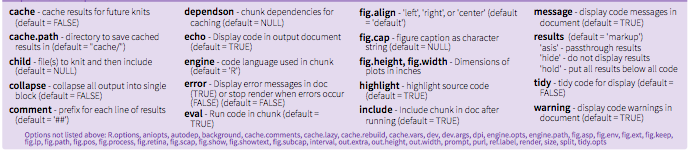
\includegraphics{chunk_parameters.png}
\caption{Parameters}
\end{figure}

\hypertarget{including-plots}{%
\subsection{Including Plots}\label{including-plots}}

You can also embed plots, for example in this case using
\texttt{echo=FALSE} only the plot will be displayed:

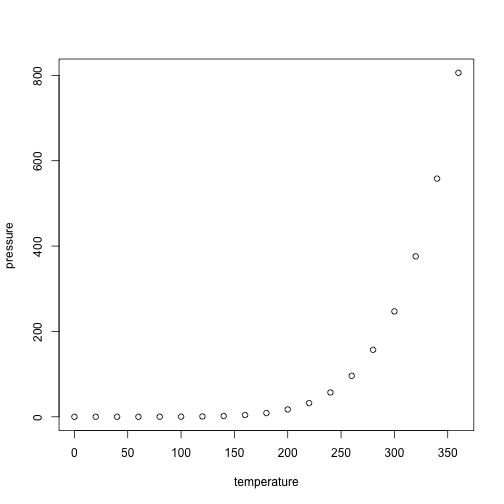
\includegraphics{markdown_tutorial_files/figure-latex/pressure-1.pdf}

Or if you have multiple plots:

\begin{verbatim}
## Sales Report {.tabset}
 
### By Product
 
(tab content)
 
### By Region
 
(tab content)
\end{verbatim}

\hypertarget{multiple-plots}{%
\subsection{Multiple plots}\label{multiple-plots}}

\hypertarget{by-class}{%
\subsubsection{By class}\label{by-class}}

\begin{Shaded}
\begin{Highlighting}[]
\NormalTok{g }\OtherTok{\textless{}{-}} \FunctionTok{ggplot}\NormalTok{(mpg, }\FunctionTok{aes}\NormalTok{(class))}
\CommentTok{\# Number of cars in each class:}
\NormalTok{g }\SpecialCharTok{+} \FunctionTok{geom\_bar}\NormalTok{()}
\end{Highlighting}
\end{Shaded}

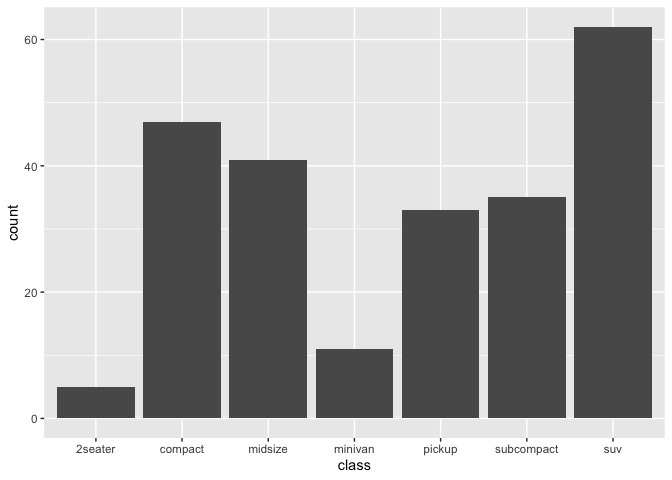
\includegraphics{markdown_tutorial_files/figure-latex/unnamed-chunk-1-1.pdf}

\hypertarget{boxplot}{%
\subsubsection{Boxplot}\label{boxplot}}

\begin{Shaded}
\begin{Highlighting}[]
\NormalTok{p }\OtherTok{\textless{}{-}} \FunctionTok{ggplot}\NormalTok{(mpg, }\FunctionTok{aes}\NormalTok{(class, hwy))}
\NormalTok{p }\SpecialCharTok{+} \FunctionTok{geom\_boxplot}\NormalTok{()}
\end{Highlighting}
\end{Shaded}

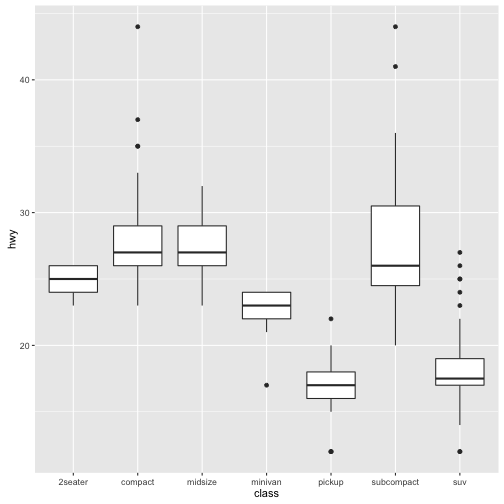
\includegraphics{markdown_tutorial_files/figure-latex/unnamed-chunk-2-1.pdf}

\hypertarget{miscelaneous}{%
\subsubsection{Miscelaneous}\label{miscelaneous}}

\begin{Shaded}
\begin{Highlighting}[]
\CommentTok{\# Extract r code}
\FunctionTok{knit}\NormalTok{(}\StringTok{"markdown\_tutorial.Rmd"}\NormalTok{, }\StringTok{"R{-}code\_markdown.R"}\NormalTok{, }\AttributeTok{tangle =} \ConstantTok{TRUE}\NormalTok{)}
\end{Highlighting}
\end{Shaded}


\end{document}
